\documentclass[a4paper, 12pt, reqno]{amsart}

\newcommand{\titl}{Actuarial Mathematics Homework 9}

\usepackage{amssymb}
\usepackage{amsfonts}
\numberwithin{equation}{section}
\usepackage[margin=1in]{geometry}
\usepackage[english]{babel}
\usepackage[colorlinks, pdftitle={\titl},
    pdfauthor={Moritz M. Konarski}]{hyperref}
\usepackage{enumitem}
\usepackage{graphicx}
\usepackage{tikz}
\usetikzlibrary{snakes}
\renewcommand{\baselinestretch}{1.25}
\usepackage{actuarialsymbol}

\title{\titl}
\author{Moritz M. Konarski}
\date{\today}

\begin{document}

\maketitle

\section*{Parmenter Exercises 4--17 to 4--25}

\subsection*{4--17}

Table:\\
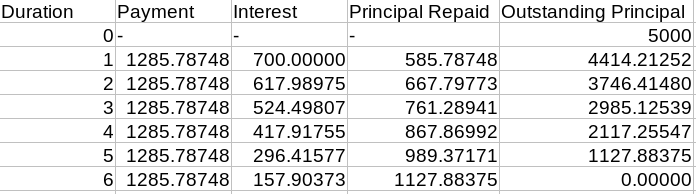
\includegraphics[width=\textwidth]{../01.png}


\subsection*{4--18}

Table:\\
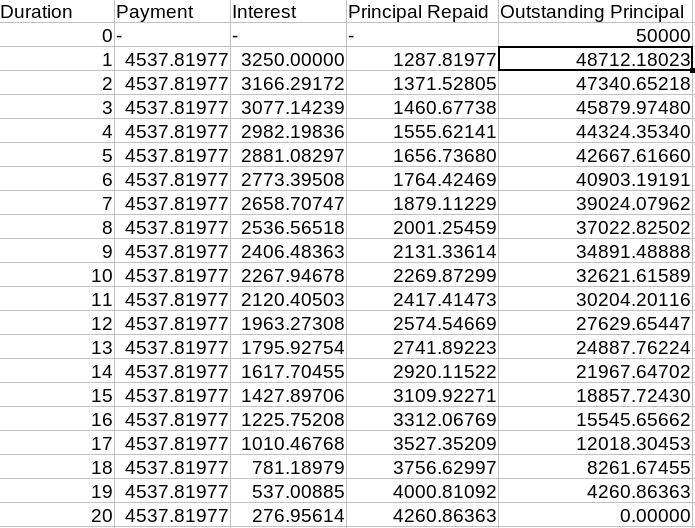
\includegraphics[width=\textwidth]{../02.png}


\subsection*{4--19}

Table:\\
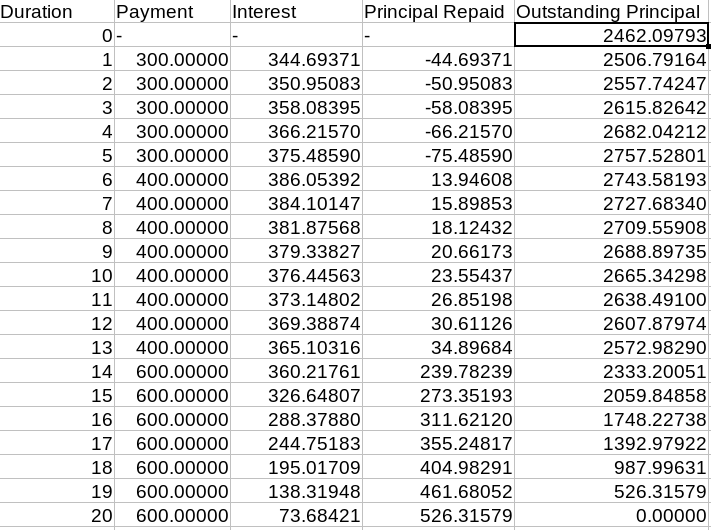
\includegraphics[width=\textwidth]{../03.png}


\subsection*{4--20}

Table:\\
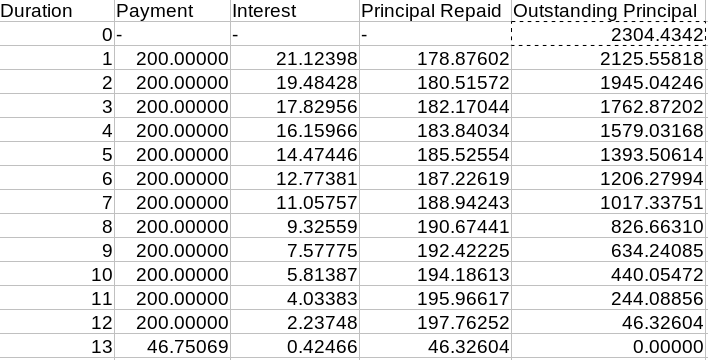
\includegraphics[width=\textwidth]{../04.png}

\subsection*{4--21}

I could not solve these problems.

\subsection*{4--22}

\begin{verbatim}
l = 5000
op = l
i = 0.14
p = 1285.78747828912

c = 0
print("Dur\tPay\t\tInt\t\tPR\t\tOP")
print("0\t-\t\t-\t\t-\t\t{0}".format(l))

while op >= 0:
    I = i * op
    pr = p - I
    op = op - pr
    c= c + 1
    print("{0}\t{1:.5f}\t\t{2:.5f}\t\t{3:.5f}\t\t{4:.5f}".format(c,p,I,pr,op))
\end{verbatim}

\subsection*{4--23}

This table has 300 rows so I will not add it here for space reasons.

\subsection*{4--24}

\begin{verbatim}
l = 2462.09793136526
op = l
i = 0.14

def get_p(c: int) -> float:
    if c < 5:
        return 300
    elif c < 13:
        return 400
    else:
        return 600

c = 0
print("Dur\tPay\t\tInt\t\tPR\t\tOP")
print("0\t-\t\t-\t\t-\t\t{0}".format(l))

while op >= 0:
    I = i * op
    pr = get_p(c) - I
    op = op - pr
    c= c + 1
    print("{0}\t{1:.5f}\t\t{2:.5f}\t\t{3:.5f}\t\t{4:.5f}".format(c,get_p(c-1),
        I,pr,op))
\end{verbatim}

\subsection*{4--25}

\begin{verbatim}
l = 2304.4342
op = l
i = 0.11/12

def get_p(c: int, op: float) -> float:
    if op > 200:
        return 200
    else:
        return op * (1+i)

c = 0
print("Dur\tPay\t\tInt\t\tPR\t\tOP")
print("0\t-\t\t-\t\t-\t\t{0}".format(l))

while op >= 0:
    I = i * op
    pr = get_p(c, op) - I
    op = op - pr
    c= c + 1
    print("{0}\t{1:.5f}\t\t{2:.5f}\t\t{3:.5f}\t\t{4:.5f}".format(c, get_p(c-1,
        op+pr), I, pr,
        op))
\end{verbatim}

\end{document}
